% Template for the submittion to:
%   The Annals of Probability           [aop]
%   The Annals of Applied Probability   [aap]
%   The Annals of Statistics            [aos]
%
%Author: In this template, the places where you need to add information
%        (or delete line) are indicated by {???}.  Mostly the information
%        required is obvious, but some explanations are given in lines starting
%Author:
%All other lines should be ignored.  After editing, there should be
%no instances of ??? after this line.

% use option [preprint] to remove info line at bottom
% journal options: aop,aap,aos
%\documentclass[aos]{imsart}
\documentclass{imsart}

\usepackage{amsthm,amsmath,natbib}
%\RequirePackage[dvips]{hyperref}

% use this package if hyperref and natbib is used:
%\RequirePackage{hypernat}

% provide arXiv number if available:
%\arxiv{math.PR/0000000}

% put your definitions there:
\startlocaldefs

\usepackage{graphics,amssymb,color}
\usepackage{graphicx,subfigure}
\usepackage[boxed]{algorithm2e}

\newcommand{\argmax}{\mathop{\mathrm{argmax}}}
\newcommand{\argmin}{\mathop{\mathrm{argmin}}}
\newcommand{\minimize}{\mathop{\mathrm{minimize}}}
\newcommand{\maximize}{\mathop{\mathrm{maximize}}}

\newcommand{\todo}{\textcolor{red}{\textbf{To do: }}}

\newcommand{\real}{\mathbb{R}}
\newcommand{\Pp}{{\mathbb P}}
\newcommand{\Ee}{{\mathbb E}}
\newcommand{\lips}{{\cal L}}
\newcommand{\tube}{\mathrm{Tube}}
\newcommand{\sphere}[1]{O^{#1-1}}
\newcommand{\dimens}{\text{dim}}
\newcommand{\cone}{\text{Cone}}
\newtheorem{theorem}{Theorem}
\newtheorem{lemma}[theorem]{Lemma}
\newtheorem{cor}[theorem]{Corollary}
\newcommand{\XK}{K_X}
\newcommand{\norm}[1]{\lVert #1 \rVert}
\newcommand{\innerp}[2]{\langle #1 , #2 \rangle}
%\newcommand{\qed}{\hfill $\Box$\newline}

\newcommand{\grad}{\nabla}
\newcommand{\V}{\mathcal{V}}\endlocaldefs
\newcommand{\K}{\mathcal{K}}
\newcommand\tf{\widetilde{f}}
\newcommand{\pen}{\mathcal{P}}

\begin{document}

\begin{frontmatter}

% "Title of the paper"
\title{A significance test in forward stepwise model selection}

%%%
%%% \runtitle{} - I don't know what this is
%%%

% indicate corresponding author with \corref{}
\author{\fnms{Jonathan} \snm{Taylor}\corref{Jonathan E. Taylor}\ead[label=e1]{jonathan.taylor@stanford.edu}\thanksref{t1}
\and \fnms{Joshua} \snm{Loftus}
\and ???}
\thankstext{t1}{Supported in part by NSF grant DMS 1208857 and
AFOSR grant 113039.}

\affiliation{Stanford University}

\address{Department of Statistics\\  Stanford University\\ Sequoia
Hall \\390 Serra Mall\\ Stanford, CA 94305, U.S.A.\\ \printead{e1}}

%%%
%%% \runauthor{Taylor} - I don't know what this is
%%%

\begin{abstract}
% perhaps de-emphasize group lasso and emphasize forward stepwise?
  We apply the methods of \cite{tests:adaptive} and
  \cite{significance:lasso} on significance tests for penalized
  regression to forward stepwise model selection. For the $k$th
  variable to enter the model, previous work relied on an asymptotic
  null distribution that breaks down when grouped variables are
  entering the model and is difficult to derive. We iteratively apply
  an exact null distribution for the first (potentially grouped)
  variable on the residual from previous steps. The resulting method
  has the strengths of stepwise selection, for example parallel
  computation, but also remedies the problem of inflated test
  statistics and over-fitting.
\end{abstract}

%%%
%%% - Gotta change these
%%%
\begin{keyword}[class=AMS]
\kwd[Primary ]{62M40}
%\kwd{}
\kwd[; secondary ]{62H35}
\end{keyword}

\begin{keyword}
\kwd{penalized regression}
\kwd{convex analysis}
\kwd{least squares}
\kwd{Gaussian processes}
%\kwd{extreme value theory}
\end{keyword}

\end{frontmatter}


\section{Introduction}
\label{sec:intro}

Forward stepwise regression is a stochastic model selection procedure
that begins with an empty model and adds the best predictor variable
in each step.  Classical significance tests fail when a model has been
selected this way and tend to be anti-conservative.  Recently,
\cite{significance:lasso} found a novel test statistic with an
appropriate null distribution that behaves well when a model has been
selected using the lasso \citep{tibshirani:lasso}.
\cite{tests:adaptive} modified and extended those results to the
group lasso \citep{grouplasso} and other adaptive regression
problems.  The present work explores the behavior of those test
statistics for models selected by forward stepwise procedures and
works out some of the details involved in applying these methods to
models with grouped variables.  Our test statistic can be
used for valid significance testing when computed from the same
data as the model selection.  The resulting method can
be more statistically efficient than validation on held-out data, and
also more computationally efficient than penalized methods with
regularization parameters chosen by cross-validation.



(\todo Change this paragraph as the sections are completed)
In Section \ref{sec:stepwise} we establish notation and describe our
forward stepwise procedure. Section \ref{sec:testing} briefly reviews
the parts of \cite{significance:lasso} and \cite{tests:adaptive}
relevant to our significance test, and describes the group lasso which
we require for applying the test with grouped
variables. Simulation results in Section \ref{sec:simulations} using
various stopping rules for the forward stepwise procedure--including
some from \cite{sequential:fdr}--appear promising.

%%%%%%%%%%%%%%%%%%%%%%%%%%%%%%%%%%%%%%%%%%%%%%%%%%%%
%%%%%%%%%%%%%%%%%%%%%%%%%%%%%%%%%%%%%%%%%%%%%%%%%%%%
%%%%%%%%%%%%%%%%%%%%%%%%%%%%%%%%%%%%%%%%%%%%%%%%%%%%

\section{Forward stepwise model selection}
\label{sec:stepwise}

We allow forward stepwise selection to add groups of variables in each
step, not only in the case of binary encoding for categorical
variables but also for any grouping purpose. For example, groups of
variables may be pre-designated factors such as expression
measurements for all genes in a single functional pathway. An entire
group is included or excluded together from the final model. For
consistency we will use $g, h$ as indices rather than the usual $i, j$
throughout. Since single variables can be considered groups of size 1,
our general exposition includes non-grouped situations as a special
case. Our variant of forward stepwise uses a different method than
usual for choosing which group to add because we are using the
same objective in the forward stepwise procedure that was used to
derive our test statistic.

Label the outcome variable of $n$ i.i.d. measurements $y \in \real^n$. Let an integer $G \geq 1$ 
be the number of groups. For each $1 \leq g \leq G$ the design matrix encoding the
$g$th group is the $n \times p_g$ matrix denoted $X_g$, where $p_g$ is
the number of individual variables in group $g$. Define $p = \sum_{g=1}^G
p_g$ the total number of individual variables, so $p = G$ in the
case where all groups have size 1. Let $X$ be the matrix constructed
by column-binding the $X_g$, that is  
%Throughout most of this paper we assume orthogonality within groups, that is
%$X_g^T X_g = I_{p_g \times p_g}$ for all $g$. ( \todo Take this out if
%we don't actually need it).  
%%%%%%%%%%%%%%%%%%%%%%%%%%%%%%%%%%%%%%%%%%%%%%%%
\begin{equation*}
X = \begin{pmatrix} X_1 & X_2 & \cdots & X_G  \end{pmatrix}
\end{equation*}
%%%%%%%%%%%%%%%%%%%%%%%%%%%%%%%%%%%%%%%%%%%%%%%%
With each group we associate the $p_g \times 1$ coefficient vector
$\beta_g$, and write $\beta$ for the $p \times 1$ vector constructed
by stacking all of the $\beta_g$ in order.  Finally, our model for the
response is
%%%%%%%%%%%%%%%%%%%%%%%%%%%%%%%%%%%%%%%%%%%%%%%%
\begin{equation}
\begin{aligned}
\label{eq:gmodel}
y & = X \beta + \sigma \epsilon \\
   & = \sum_{g=1}^G X_g \beta_g + \sigma \epsilon
\end{aligned}
\end{equation}
%%%%%%%%%%%%%%%%%%%%%%%%%%%%%%%%%%%%%%%%%%%%%%%%
where $\epsilon$ is noise. Unless otherwise specified we assume
i.i.d. Gaussian noise $\epsilon \sim N(0, I_{n \times n})$ and that
$\sigma$ is known.

We allow for the possibility $p > n$ in which case ~\ref{eq:gmodel} is
generically underdetermined. In such cases it still may be possible to
estimate $\beta$ well if it is sparse--that is, if it has few nonzero
entries \citep{donoho:pursuit}. In the rest of this paper we refer to
variable groups $X_g$ as noise variables if $\beta_g$ is a zero vector
and as true predictor variables if $\beta_g$ has nonzero entries.

Before we describe the forward stepwise procedure we require one last
ingredient. To each group of variables we assign a weight $w_g$. These
weights act like penalties or costs, so increasing $w_g$ makes it
more difficult for the group $X_g$ to enter the model. The
modeler can choose weights arbitrarily, but we will only use one
particular choice, based on $p_g$, that we discuss later. With this we
are ready to describe the forward stepwise procedure, given in Algorithm
\ref{algo:fs}. Note that to enable our p-value computations,
\textit{max.steps} should be at most $\min (n, G) - 1$. If the noise
variance is known--as we assume unless specified otherwise--and
$\beta$ is expected to be quite sparse, then \textit{max.steps} can be
much smaller as long as it is still above the expected sparsity of
$\beta$. This last constraint is suggested so that forward stepwise
still has a chance of recovering all the nonzero coefficients of
$\beta$ before reaching \textit{max.steps}. In our implementation we
treat the active set $A$ as an ordered set to easily track the order
of variables entering the model.

\begin{algorithm}
\DontPrintSemicolon
\KwData{An $n$ vector $y$ and $n \times p$ matrix $X$ of $G$ grouped variables}
\KwResult{Active set $A$ of variable groups included in the model}
\SetKwFunction{lsfitResidual}{lsfitResidual}
\caption{Forward stepwise procedure with groups and weights}
\BlankLine
$A \gets \emptyset$\;
$A^c \gets \{ 1, \ldots, G \}$\;
$r_0 \gets y$\;
\For{$s \gets 1$ \KwTo $max.steps$}{
  $g^* \gets \argmax_{g \in A^c} \{ \norm{X_g^T r_{s-1}}_2 / w_g \}$\;
  $P \gets I - X_{g^*}X_{g^*}^\dagger$\;
  $A \gets A \cup \{ g^* \}$\;
  $A^c \gets A^c \backslash \{ g^* \}$\;
  \For{$g \in A^c$}{
    $X_g \gets P X_g$\;
  }
  $r_s \gets P r_{s-1}$\;
}
\KwRet{$A$}
\label{algo:fs}
\end{algorithm}


Subset selection refers to the problem of choosing a subset of the $G$
potential groups to include in a model. Since there are $2^G$ such
choices, exhaustive search is computationally infeasible when $G$ is
large. If exhaustive search were possible, performing a large
search runs the risk of over-fitting unless model complexity is
appropriately penalized. Forward stepwise produces a much
smaller set of potential models, with cardinality at most \textit{max.steps}. However,
it is a greedy algorithm so the set of models it produces may not
contain the best possible model. This is an inherent shortcoming of
forward stepwise procedures and should be kept in mind when choosing
between model selection methods.

So far we have left open the question of choosing among the models in
the forward stepwise sequence, i.e. when to stop stepping
forward. Some classical approaches can be posed as optimization
criteria which stop at the step minimizing
\begin{equation}
\begin{aligned}
\label{eq:subsetregress}
\frac{1}{2} \| y - X \beta_s \|_2^2 + \lambda \pen(\beta_s)
\end{aligned}
\end{equation}
where we have written $\{ \beta_s : s = 1, \ldots, max.steps \}$ as
the sequence of models outputted by forward stepwise. The function
$\pen(\beta)$ is a penalty on model complexity usually taken to be the
number of nonzero entries of $\beta$. Proposals for $\lambda$ include
2 ($C_p$ of \cite{CP}, AIC of \cite{AIC}), $\log(n)$ (BIC of \cite{BIC}), and
$2\log(p)$ (RIC of \cite{RIC}). In the current paper we provide
accurate p-values when adding the first noise variable group in the forward
stepwise sequence, and it is natural to consider using these p-values
to choose a model. \cite{sequential:fdr} examined some stopping rules
using the asymptotic p-values of \cite{significance:lasso} and showed
their stopping rules control false discovery rate--the expected
proportion of noise variables among variables declared significant
\citep{fdr}. We explore this further in Section \ref{sec:simulations}.

Although forward stepwise is a greedy algorithm producing a
potentially sub-optimal sequence of models, under favorable conditions
it can still perform well. There is a parallel literature to the
compressed sensing literature \textit{(cite some here)} with theorems
stating that forward stepwise can exactly select the true model under
some stringent conditions involving quantities like the sparsity of
the true model and the coherence of the design matrix. Recall that the
coherence $\mu(X)$ of a matrix $X$ with columns scaled to have unit
2-norm is defined as

\begin{equation}
  \mu(X) = \max_{i \neq j} \{ | \innerp{ X_i }{ X_j } | \}
\end{equation}

Writing $k$ for the sparsity of $\beta$, typical results in this
literature say that if $k < (1/\mu + 1)/2$ and the nonzero
coefficients of $\beta$ are sufficiently large then forward stepwise
recovers $\beta$ with high probability. We refer the
reader to the literature for details. For our purposes the
conditions required to guarantee exact recovery are usually far too
stringent. We conduct simulations to show empirically that forward
stepwise can work well even when it is not working perfectly, and that
it does so under a much wider range of conditions.


\begin{figure}
\begin{center}
\subfigure[Ternary design]{
\label{fig:fsternary}
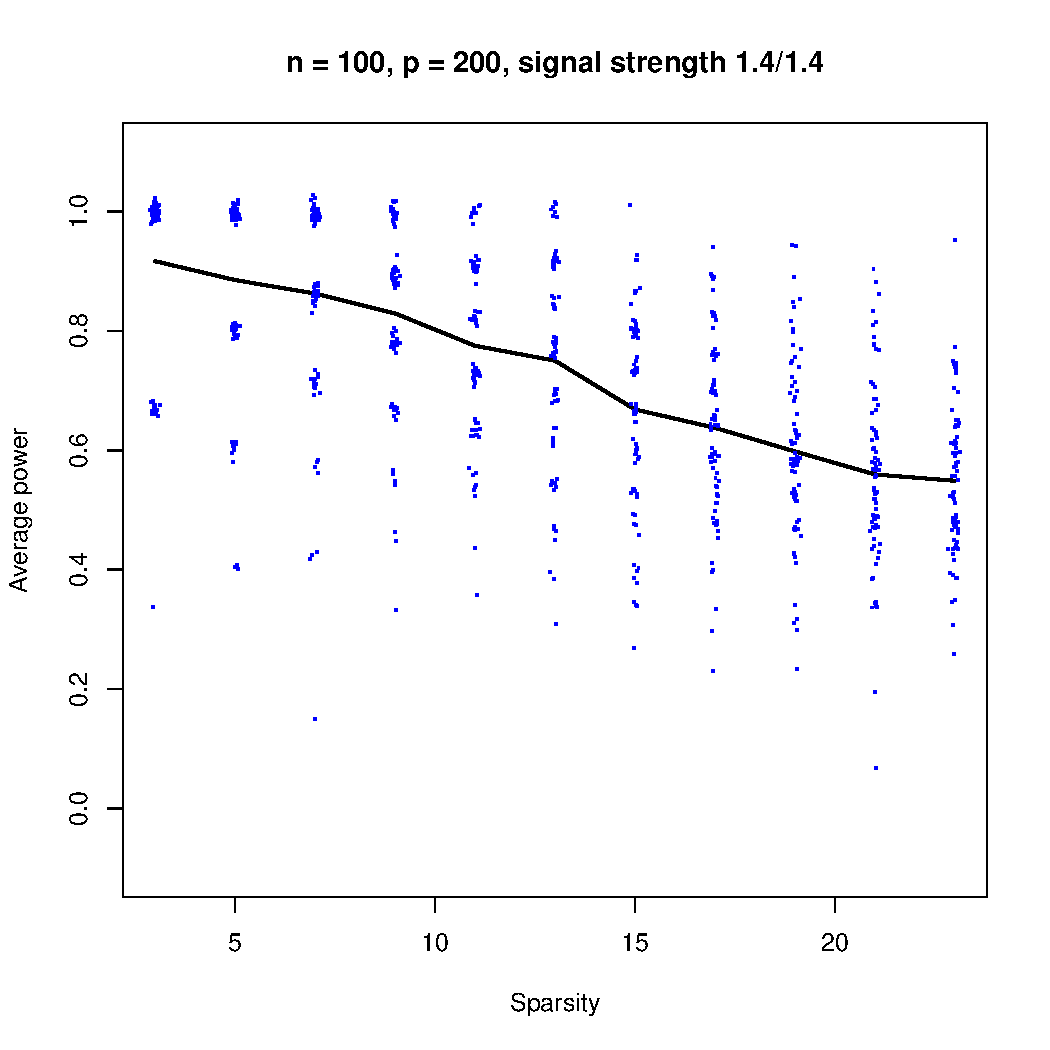
\includegraphics[width=0.5\textwidth]{../figs/fwdstep/ternary_p2n_n100_lower1p4_upper1p4.pdf}}
\hspace{-15pt}
\subfigure[Gaussian design with correlation]{
\label{fig:fsgausscorr}
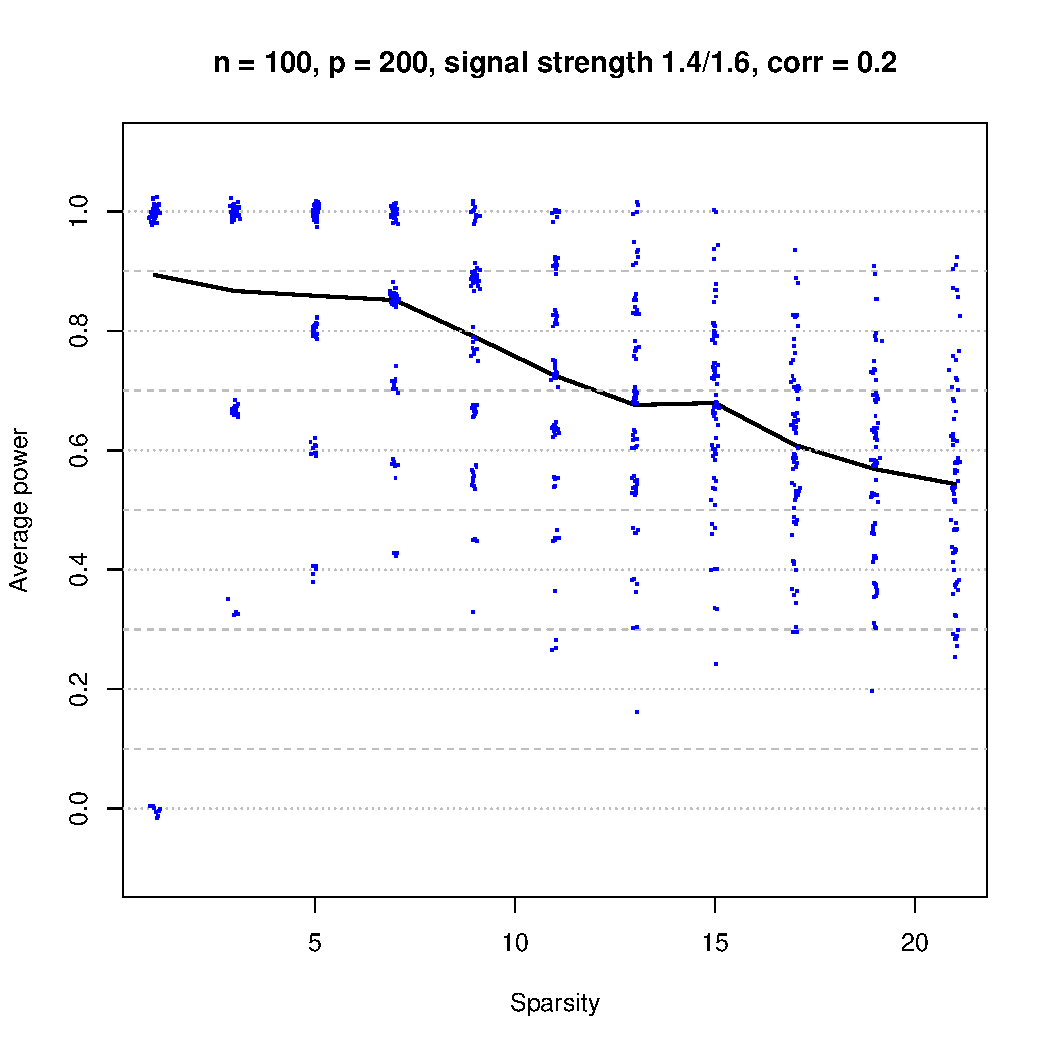
\includegraphics[width=0.5\textwidth]{../figs/fwdstep/gaussian_p2n_n100_lower1p4_upper1p6_corr0p2.pdf}}
\caption{\small \it The left panel shows the results of the simulation
  using design matrices with i.i.d. ternary entries taking values $0,
  \pm 1$ with equal probability. The left panel shows the results
  with design matrices of standard Gaussian entries with
  equi-correlation of 0.2. }
\label{fig:fwdstepsim}
\end{center}
\end{figure}

For various sparsity levels $k$, Algorithm ~\ref{algo:fs} was run on
various data sets with max.steps equal to $k$ and the ``average
power'' was calculated as the number of true variables in the active
set after $k$ steps divided by $k$. Nonzero coefficients had magnitude
in a range of multiples of $\sqrt{2\log(p)}$, e.g. in $[1.4
\sqrt{2\log(p)}, 1.6 \sqrt{2\log(p)}]$. Results are shown in
Figure~\ref{fig:fwdstepsim}. Some calculations show the required
sparsity level to guarantee exact recovery in these situations is
about 2 or smaller, and the required nonzero coefficient magnitude is
likely in the range of 10 to 100 times $\sqrt{2\log(p)}$. 

%%%%%%%%%%%%%%%%%%%%%%%%%
%%%%%%%%%%%%%%%%%%%%%%%%%

\section{Significance testing: from lasso to group lasso}
\label{sec:testing}

\todo Update this section to match/complement \citep{tests:adaptive}



In the ordinary least squares setting, a significance test for a
single variable can be conducted by comparing the drop in residual
sums of squares (RSS) to a $\chi^2_1$ distribution. Similarly, when
adding a group of $k$ variables we can compare the drop in RSS to a
$\chi^2_k$ random variable. This generally does not work when the
variable to be added has been chosen by a method that uses the data,
and in particular it fails for forward stepwise procedures adding
the ``best'' (e.g. most highly correlated) predictor in each step. In
that case, the test statistic (drop in RSS) does not match the
theoretical null distribution even when the null hypothesis is
true. \cite{significance:lasso} introduced a new test statistic based
on the knots in the lasso solution path. They derived a simple
asymptotic null distribution, proved a type of convergence under broad
``minimum growth'' conditions, and demonstrated in simulations that
the test statistic closely matches its asymptotic distribution even in
finite samples.  That work marked an important advance in the problem
of combining inference with model selection.  The current paper
extends some of their results to the group lasso \citep{grouplasso}.
In the process we had to derive an exact finite sample null
distribution for the test statistic, this appears in
\cite{tests:adaptive}. 


Writing $\hat \beta(\lambda)$ for the lasso solution for a fixed value of $\lambda$, we need
the following facts summarized in \cite{significance:lasso} (ref Tibs2012?).

\begin{itemize}

  \item The vector valued function $\hat \beta(\lambda)$ is a
    continuous function of $\lambda$. For the lasso path, the
    coordinates of $\hat \beta(\lambda)$ are piecewise linear with
    changes in slope occurring at a finite number of $\lambda$ values
    referred to as \emph{knots}. The knots depend on the data and are
    usually written in order $\lambda_1 \geq \lambda_2 \geq \cdots
    \geq \lambda_r \geq 0$. We follow this convention. 

  \item The \emph{active set} $A_k$ is a set of indices of variables
    for which the corresponding coordinates of $\hat \beta(\lambda_k)$
    are potentially nonzero. Any variable with index not in $A_k$ has
    a zero coefficient in $\hat \beta(\lambda_k)$, but the converse is
    not true. \todo{is this equicorrelation set?}
  
  \item Path algorithms for computing lasso solutions proceed by
    fitting models at a grid of $\lambda$ values. The active set
    changes whenever $\lambda$ crosses a knot, and predictor variables
    can both enter and leave the active set. However, at the first two
    knots $\lambda_1$ and $\lambda_2$ no variable can leave the active
    set. So the first two knots correspond to the first two variables
    entering the model. 

\end{itemize}

\cite{significance:lasso} prove that under the null hypothesis that $A_k$
contains all the strong predictor variables, the distribution of a
test statistic $T_k \propto \lambda_k(\lambda_k - \lambda_{k+1})$ is
asymptotically Exp(1). In the lasso case we know a lot about the knots
and active set, but the group lasso picture is slightly more
complicated. For the group lasso, $\hat \beta(\lambda)$ does not have
piecewise linear components. To overcome this difficulty we will
restrict our attention to the first group of variables to enter the
active set since the analysis then follows almost exactly as for the
lasso.

The \emph{group lasso estimator} is a solution to the following convex
problem
%%%%%%%%%%%%%%%%%%%%%%%%%%%%%%%%%%%%%%%%%%%%%%%%
\begin{equation}
\begin{aligned}
\label{eq:gsoln}
\displaystyle \hat \beta_\lambda = \argmin_{\beta \in \real^p} \frac{1}{2} \| y - X \beta \|_2^2 +
   \lambda \sum_{g=1}^G w_g \| \beta_g \|_2
\end{aligned}
\end{equation}
%%%%%%%%%%%%%%%%%%%%%%%%%%%%%%%%%%%%%%%%%%%%%%%%
The parameter $\lambda \geq 0$ enforces sparsity in groups: for large
$\lambda$ most of the $\beta_g$ will be zero vectors. The weights
$w_g$ are usually taken to be $\sqrt p_g$ to normalize the penalty
across groups.  Note that this includes the usual lasso estimator as a
special case when all of the groups are of size 1, since then the
penalty term is the $L^1$-norm of $\beta$. 

%%%%%%%%%%%%%%%%%%%%%%%%%%%%%%%%%%%%%%%%%%%%%%%%
%%%%%%%%%%%%%%%% Related works %%%%%%%%%%%%%%%%%
%%%%%%%%%%%%%%%%%%%%%%%%%%%%%%%%%%%%%%%%%%%%%%%%

\todo Fix references below

The group lasso estimator is discussed in (ref that guy's thesis) and
(ref Yuan and Lin).  An important extension is the sparse group lasso
(ref ???) which enforces sparsity in groups as well as sparsity of the
coefficients within the groups.  For a survey on group lasso and
related factor models see (ref???). \todo review some more literature
and add a few more references here if they seem worthwhile. 


Before considering the group lasso, we review some ingredients of the
proof for the lasso. Let $J = \{ 1, 2, \ldots, p \}$ index variables
and consider a stochastic process $f_{j,s} = sX_j^Ty$ defined on $T =
J \times [ -1, 1 ]$. This stochastic process is simply a collection of
linear combinations of $y$, hence it is Gaussian under the assumption
of Gaussian errors. The \emph{Karush-Kuhn-Tuckher (KKT) conditions}
(ref???) imply that $\lambda_1 = \max_j |X_j^Ty|$. By introducing the
sign variable $s$, we can remove the absolute value and write
$\lambda_1$ as the maximum of our Gaussian process 

\begin{equation}
\lambda_1 = \max_{(j,s)} f_{j,s}
\end{equation}

We have exhibited the first knot as the maximum of a Gaussian
process. We can do this for the second knot by introducing a new
process. Let $(j_1, s_1)$ be the maximizer so that $\lambda_1 =
s_1X_{j_1}^Ty$, and define 
%%%%%%%%%%%%%%%%%%%%%%%%%%%%%%%%%%%%%%%%%%%%%%%%
\begin{equation}
\begin{aligned}
  f^{(j_1,s_1)}_{(j,s)} & = \frac{ sX_j^T y - s X_j^T X_{j_1} X_{j_1}^Ty  } { 1 -  ss_1 X_j^TX_{j_1}} \\
  & = \frac{ sX_j^T(I-P_{j_1}) y }{ 1 -  s_1 X_{j_1}^T X_js}
\end{aligned}
\end{equation}
%%%%%%%%%%%%%%%%%%%%%%%%%%%%%%%%%%%%%%%%%%%%%%%%
where $P_j$ is the projection onto the subspace spanned by $X_j$. We
can think of this as a ``residual process'' after regressing out the
maximum. Write $M = \max_{j \neq j_1, s} f^{(j_1,s_1)}_{(j,s)}$, the
maximum of this residual process. It can be shown from the KKT
conditions that $M  = \lambda_2$. To summarize, we have represented
the first two knots of the lasso solution path as the maxima of some
natural Gaussian processes. Distributional facts about Gaussian
processes now allow us to make conclusions about the distribution of
functions of the knots. 

\subsection{Group lasso}
To extend this argument to the group lasso we need to define Gaussian
processes that characterize the knots of the group lasso solution
path.  

\todo Either use the simplified argument in the case of equal weights
(equal group sizes), or finish adjusting the proof of $M = \lambda_2$
to include the weights and use that version. The proof can go in an
appendix. 

\todo Modify write-up to match notation with \cite{tests:adaptive} and
then paste it in here

\subsection{Better p-values}

Maybe just reference \cite{tests:adaptive}? It might be worthwhile to
leave in the connection with \cite{significance:lasso} (getting our
test statistic by not using the approximation)

\begin{itemize}

\item \todo Add the figures to this section
\item \todo Convert to exposition instead of bulleted list
\item \todo Update to reflect latest work
  \item As in LTTT, $T = \lambda_1 (\lambda_1 - M)$ and $M = \lambda_2$
  \item Convergence to the limiting Exp(1) distribution is too slow
    \[
      \frac{P(\chi_k / w_g \geq m + t/m)}{P(\chi_k / w_g \geq m)} \to e^{-t} \text{ as } m \to \infty
    \]
    (when the group achieving $\lambda_1$ is group $g$ and has rank $k$)
  \item The limiting distribution only depends on $T$, but we also observe $M$
  \item Let's just try the ratio (conditional $\chi_k$ tail probability) evaluated at $T$ and $M$ (it works better)
  \item Going one step further, instead of using the approximation (see LTTT Proof of Lemma 5)
    \[
      \frac{M + \sqrt{M^2+4t}}{2} \approx M + \frac{t}{M}
    \]
    we can just use the left hand side
  \item For $T = \lambda_1(\lambda_1 - M)$ the left hand side simplifies to $\lambda_1$
  \item Now our p-value is
    \[
      \frac{P(\chi_k / w_g \geq \lambda_1)}{P(\chi_k / w_g \geq \lambda_2)}
    \]   
\end{itemize}



\section{Simulations}
\label{sec:simulations}

\todo Expand, include simulation results (copy latex for
includegraphics etc), do the simulation comparing stopping rules

\begin{itemize}
  \item Show null and non-null p-value-by-step plots for several examples
  \item Discuss one of these carefully (perhaps with a noise variable
    entering before a signal variable), for several fixed stopping points
  \item Compare a few stopping rules, e.g. naive one(s),
    TailStop/HybridStop, AIC/BIC/Cp
  \item (the stopping comparisons are not done yet, but I am guessing
    they will be comparable, perhaps AIC/BIC/Cp will be better, and in
    that case look for other advantages of ours to mention,
    e.g. interpretability for being based on p-values rather than a
    complexity penalty)

\end{itemize}


\begin{figure}
\begin{center}
\subfigure[Gaussian design]{
\label{fig:smallgauss}
\includegraphics[width=0.5\textwidth]{../figs/gaussian_size1_n100_p200_g200_k10_lower1p8_upper1p9.pdf}}
\hspace{-15pt}
\subfigure[Categorical design]{
\label{fig:smallcat}
\includegraphics[width=0.5\textwidth]{../figs/gaussian_size1_n100_p200_g200_k10_lower1p8_upper1p9_corr0p1.pdf}}
\caption{\small \it The left panel shows results of a simulation with
  an independent Gaussian design matrix and a signal vector having
  three groups with non-zero coefficients of sizes one, two, and
  three, and seven groups of noise variables with sizes varying from
  one to ten, for a total of 30 variables. For the right panel we
  repeated this setup, but group sizes corresponded to levels of
  categorical variables. The groups of size one were increased to two,
so there are 10 categorical variables with a total of 32 levels.}
\end{center}
\end{figure}



\input{../small_sim_selection.tex}

\input{../small_sim_estimation.tex}

\begin{figure}
\begin{center}
\subfigure[Large Gaussian lasso]{
\label{fig:largelasso}
\includegraphics[width=0.5\textwidth]{../figs/gaussian_size5-10_n100_p200_g35_k10_lower1p8_upper1p9.pdf}}
\hspace{-15pt}
\subfigure[Large Gaussian group lasso]{
\label{fig:largegrplasso}
\includegraphics[width=0.5\textwidth]{../figs/gaussian_size5-10_n100_p200_g35_k10_lower1p8_upper1p9_corr0p1.pdf}}
\caption{\small \it The left panel shows results of a simulation with
  an independent Gaussian design matrix and a signal vector having
  three groups with non-zero coefficients of sizes one, two, and
  three, and seven groups of noise variables with sizes varying from
  one to ten, for a total of 30 variables. For the right panel we
  repeated this setup, but group sizes corresponded to levels of
  categorical variables. The groups of size one were increased to two,
so there are 10 categorical variables with a total of 32 levels.}
\end{center}
\end{figure}

\input{../large_sim_selection.tex}

The large simulation has 50 groups, 25 of size 1, 10 of size 5, 10 of
size 10, and 5 of size 15. Signal vectors were supported on random
choices of 10 of these groups (changing in each realization), with
non-zero signal magnitude around $\sqrt{2\log p}$ where $p = 250$
(roughly 3.3). The design matrix had 200 rows and the simulation
performed 100 realizations.



\section{Real data example}
\todo Simulation with non-Gaussian design matrix (from AIDS data probably)



\section{Discussion}
\label{sec:discuss}

\todo After finising everything else, move some points of discussion
here, re-read and see if there's anything else interesting to comment
on here. Mention ongoing work

\bibliographystyle{ims}
%\bibliographystyle{acmtrans-ims}
\bibliography{paper}


\appendix
\section{Derivation of closed forms of statistic}

For the sake of completeness this appendix provides full derivations
of closed forms for the quantities required to compute our
statistic. We require two facts from \cite{tests:adaptive}

A point $\eta \in \K$ maximizes $f_\eta$ over a convex
set $\K$ if and only if the following conditions hold: 
\begin{equation}
\label{eq:maxcond}
\grad f_{|T_{\eta}\K} = 0, \quad
\tf^{\eta}_{\eta} \geq \V^+_{\eta}, \quad
\tf^{\eta}_{\eta} \leq \V^-_{\eta}, \quad \text{and} \quad
\V^0_{\eta} \leq 0.
\end{equation}
The same equivalence holds true even when $\K$ is only locally
convex. 

Write $M^{\pm}_{\eta, h}$ and $M^0_{\eta, h}$ as the corresponding suprema and infima over the restricted parameter set $S_h$. Note that the characterization of the global maximizer (Lemma 1, general paper) implies $M^0_{\eta, h} \leq 0$ and $M^+_{\eta, h} \leq M^-_{\eta, h}$ for all $h \neq g$. This will be used below to eliminate some degenerate cases of the optimization sub-problem on each $S_h$.

Now fix $h$, let $P_g = X_gX_g^T$ and define
\begin{align*}
a_h &= w_h^{-1} X_h^T (I-P_g) y \\
b_h &= w_g w_h^{-1} X_h^T P_g y / \norm{X_g^T y} \\
c_h &= a_h^T b_h / (\norm{a_h} \norm{b_h}) \\
K_h   &= \{ x : \norm{x} = 1, b_h^Tx > w \}
\end{align*}
Note that $K_h = \emptyset$ if and only if $\norm{b_h} < w$. We will consider two cases. First, suppose $\norm{b_h} > w$. In this case we must rule out one sub-case, when $a_h$ is not in the polar cone of $K_h$. If this occurs, then on at least one side of the boundary of $K_h$ we have $a_h^Tx > 0$ there, so that the infimum inside $K$ is $-\infty$ but the supremum outside $K$ is $+\infty$. This violates the characterization of the global maximizer of the original process as described above, so this case cannot occur.

Now, if $a_h$ is in the polar cone of $K_h$ (and ruling out the probability zero case where $a_h^Tx = 0$ on the boundary of $K_h$), then the numerator $a_h^Tx < 0$ on $K_h$ so there is a finite positive infimum in the interior $K_h$. Similarly there is a finite positive supremum on the interior of $K_h^c$ (the numerator is negative near the boundary of $K_h$ by continuity).

To attain the infimum on $K_h$ requires making $x$ close to $b_h$ and simultaneously making the numerator closer to zero, so $x$ should be on the side of $b_h$ that is closer to $a_h$. To attain the supremum on $K_h^c$ requires making $x$ simultaneously close to $a_h$ (so that $a_h^Tx > 0$) and $b_h$ (to make the denominator small). In summary, both the infimum and supremum are attained with $x$ between $a_h$ and $b_h$, when the angle $\theta$ between $a_h$ and $b_h$ is larger than both the angle $\psi$ between $a_h$ and $x$ and the angle $\phi$ between $x$ and $b_h$. This allows the simplification $\phi = \theta - \psi$. This is easier to verify for the case when $\norm{b_h} < w$.

We have verified that solving both cases requires finding the maxima of the trigonometric form $\norm{a_h} \cos (\psi) / (w - \norm{b_h} \cos(\theta - \psi))$ of the linear fraction on the interiors of $K_h$ (if it is nonempty) and $K_h^c$. The derivative is proportional to
\[
\frac{\norm{b_h} \sin(\theta) - w \sin(\psi)}{w - \norm{b_h} \cos(\theta - \psi)}
\]
Since we have ruled out the boundary of $K_h$, we can ignore the denominator and focus on critical points corresponding to the angles $\psi^{\pm}$ (symmetric about $\pi/2$) where $\sin(\psi^{\pm}) = (\norm{b_h} / w) \sin (\theta)$. That is,
\[
\psi^{\pm} \in \arcsin \frac{\norm{b_h}}{w} \sqrt{1-c_h^2}
\]
Note that these critical points only exist if $\sin(\theta) < w/\norm{b_h}$, and since we have argued that the infimum and supremum are attained it follows that this condition is met in our case. Let $\psi^+$ denote the smaller of the two angles. If $K_h$ is nonempty, then $\psi^-$ gives the infimum in $K_h$ and $\psi^+$ the supremum on $K_h^c$. This is necessary since if $x$ is in $K_h$ then its angle from $a_h$ is larger than $\pi/2$ because $a_h$ is in the polar cone of $K_h$. If $K_h$ is empty, then the supremum is still attained at $\psi^+$ since the numerator is negative at $\psi^- > \pi/2$ and the denominator is always positive.

Finally we calculate the values of the linear fraction at $\psi^{\pm}$. Let us first record some facts:
\begin{align*}
0 < \psi^+ < \pi/2, \quad \psi^- = \pi - \psi^+ \\
\cos(\theta) = c_h, \quad \sin(\theta) = \sqrt{1-c_h^2} \\
\sin(\psi^+) = \sin(\psi^-) = \frac{\norm{b_h}}{w} \sin(\theta) \\
\cos(\psi^+) = -\cos(\psi^-) = \sqrt{1 - (\norm{b_h}/w)^2(1-c_h^2)}
\end{align*}
Using the angle difference formula,
\begin{align*}
\cos(\theta - \psi^+) & = \frac{\norm{b_h}}{w} (1-c_h^2) +  c_h \cos(\psi^+) \\
& = \frac{\norm{b_h}}{w} (1-c_h^2) +  c_h \cos(\psi^+)
\end{align*}
Hence
\begin{align*}
M^+_{\eta, h} & = \frac{ \norm{a_h} c_h }{ w - (\norm{b_h}^2/w) (1-c_h^2) - \norm{b_h} c_h \cos(\psi^+) } \\
% & = 
% & = \frac{ w \norm{a} a_h^Tb_h / \norm{b_h} }{ w^2 - \norm{a}\norm{b}^2 + (a^Tb)/\norm{a} - a^Tb \cos \psi^+ }
\end{align*}
And $M^-_{\eta, h}$ is $\infty$ when $\norm{b_h} < w$ and otherwise given by
\begin{align*}
M^+_{\eta, h} & = \frac{ \norm{a_h} c_h }{ w - (\norm{b_h}^2/w) (1-c_h^2) + \norm{b_h} c_h \cos(\psi^+) } \\
\end{align*}

I haven't been able to algebraically simplify these yet to a form that allows my $\lambda_2$ proof below to go through. The version below just assumes $\norm{b_h} < w = 1$.

\hrule
\hrule
We can rewrite this by rationalizing the denominator:
\[
M =
\frac
{ a_h^T b_h +  \sqrt{ a_h^T a_h (1-b_h^Tb_h) + (a_h^T b_h)^2 }  }
{ 1-b_h^Tb_h }
\]
Leaving $M$ in this form we now consider $\lambda_2$. The KKT conditions for the group lasso problem give (directly from Yuan and Lin)
\begin{align*}
\norm{ X_g^T(y - X \beta) } & \leq \lambda w_g \quad \forall \beta_g \neq 0 \\
\beta_g & = \left( 1 - \frac{ \lambda w_g }{ \norm{S_g} } \right)_+ S_g
\end{align*}
where $S_g = X_g^T(y - X \beta_{-g})$. These expressions simplify for $\lambda_2 \leq \lambda < \lambda_1$. Letting $g$ be the index of the first group to enter we now have $S_g = X_g^Ty$ 
\begin{align*}
\beta_g & = \left( 1 - \frac{ \lambda w_g }{ \norm{X_g^Ty} } \right) X_g^Ty \\
\lambda w_h & \geq \norm{ X_h^Ty - X_h^T P_g y (1-\lambda w_g / \norm{X_g^Ty})  } \quad \forall h \neq g
\end{align*}
Now let $\lambda = \lambda_2$, so the inequality above is strict for all other groups and equality is attained for the second group to enter. Hence $\lambda_2$ satisfies
\begin{align*}
\lambda_2 & = \max_{h \neq g} 
\norm{ X_h^T(I - P_g) y - \lambda_2 ( w_g X_h^T P_g y / \norm{X_g^Ty} )  } / w_h\\
& = \max_{h \neq g} \norm{ a_h - \lambda_2 b_h } 
\end{align*}

Write $\lambda_{2,h}$ as the positive root of the quadratic equation obtained by squaring the norm, so $\lambda_{2,h}^2 = \norm{ a_h - \lambda_2 b_h }^2$. Then $\lambda_2 = \max_{h \neq g} \lambda_{2,h}$. Solving this (note that $b_h^Tb_h < 1$), we find
\[
\lambda_{2,h} = \frac
{ a_h^T b_h +  \sqrt{ a_h^T a_h (1-b_h^Tb_h) + (a_h^T b_h)^2 }  }
{ 1-b_h^Tb_h }
\]
Hence when $h$ is the index of the second group to enter, we have $\lambda_2 = \lambda_{2,h} = M$.

\end{document}

